\section{Week 1}
\subsection{Objective}
The objective of this week is to explore the basics of probabilistic machine learning by implementing a Bayesian linear regression model 
and explore how it is affected by its different hyperparameters like choice of prior as well as the variance and quantity of data points.
\todo{Notes from meeting: Make 2D plot over parameter space that shows how the posterior moves from the prior. Update from Oswin's notes}
\subsection{Theory}
The linear model I've chosen to implement is based on the one described in the lecture notes for the PML course.\\ \todo{add citations. Rough draft - terminology will be revised later}
Given a dataset $\mathcal{D}$ of $\ell$ datapoints, we let each datapoint $i$ consist of a vector of controlled variables $\mathbf{x}^{(i)}$ and some target variable $y^{(i)}$. The $\mathbf{x}$'s are encoded in a $\ell \times d$ matrix $\mathcal{X}$ and the $y$'s in a $\ell$ length vector.
We are interested in finding a parameter vector $\theta$ such that for any $i$, $f_\theta(x^{(i)}) = \theta^T x^{(i)} \approx y^{(i)}$.\\
To do this, we will start by assuming that the $y$'s are generated by some latent linear model $g$ with some noise $\epsilon$:
$$y^{(i)} = g(\mathbf{x}^{(i)}) + \epsilon$$
where $\epsilon \sim \mathcal{N}(0, \sigma^2_y)$ for some $\sigma^2_y$.\\
As is standard practice in linear regression, adding an extra dimension to $\mathcal{X}$ consisting of 1's will be done such that the linear model can account for offset in the data.\\
We are interested in finding measuring how likely it is for each possible parameter vector to have generated the dataset,
which we will measure using the posterior distribution $p(\theta | \mathcal{D}) = p(\theta | \mathcal{X}, \mathcal{Y})$.
Using Bayes' rule, we can write this as:
$$p(\theta | \mathcal{X}, \mathcal{Y}) = p(\theta | \mathcal{Y}, \mathcal{X}) = \frac{p(\theta|\mathcal{X}) p(\mathcal{Y}| \theta, \mathcal{X})}{p(\mathcal{Y}|\mathcal{X})} = p(\theta | \mathcal{Y}, \mathcal{X}) = \frac{p(\theta) p(\mathcal{Y}| \theta, \mathcal{X})}{p(\mathcal{Y}|\mathcal{X})}$$
where $p(\mathcal{Y}|\mathcal{X})$ is only a normalization constant and can be ignored, since we're interested in finding which $\theta$ optimizes the posterior, not the actual value of the posterior. We also assume that $p(\theta|\mathcal{X})=p(\theta)$ since we assume that the weights of the underlying distribution are independent of the observations.\\
The prior $p(\theta|\mathcal{X})$ will be assumed to be normal such that $p(\theta | \mathcal{X}) = \mathcal{N}(\theta, \mu_\theta, \Sigma_\theta)$.\\
By our assumption of the noise $\epsilon$ being normally distributed, we can thus also assume that the likelihood $p(\mathcal{Y}|\theta, \mathcal{X})$ is normally distributed. \todo{show why likelihood is normal}
\todo{litterature says need to compute $p(\mathcal{D}, \theta)$ - find out why}
Thus the prior and likelihood are conjugate and we can assume the posterior to be normal as well. This means we can calculate the posterior exactly. \\
\textbf{insert formula here}\\
\todo{Insert formula, insert calculations for $\mu$ and $\Sigma$, text about MAP vs Mean vs Posterior Predictive etc.}
\subsection{Design}
There exists a multitude of hyperparameters that can affect the posterior distribution of the model parameters.\\
These can be controlled by the model designer and include
\begin{itemize}
  \item Choice of prior mean \todo{linear regression is invariant to translation}
    \item Choice of prior variance
    \item Choice of predictive function or distribution (MAP vs Mean vs Predictive Posterior)
\end{itemize}
The model can also be subjected to different kinds of data sets, which can vary by
\begin{itemize}
  \item Underlying distribution generating the data points
  \item Number of data points
  \item Variance of data points (i.e. magnitude of noise)
  \item Dimensionality
\end{itemize}
To study the model's behavior, I will first train the same model on multiple data sets generated by the same underlying distribution, but with different amounts of data points.
Then, I will train the model on the same amount of data generated by the same distributino, but with different amounts of noise.
Finally, I will train the model on the same data set, but with different choices of parameters for the prior.
\subsection{Results}\todo{Add section for change of noise}
\subsubsection{Varying number of data points}
\todo{Make plots nicer, add "true" line for reference, add legend}
\begin{figure}[H]
\begin{subfigure}{.5\textwidth}
  \centering
  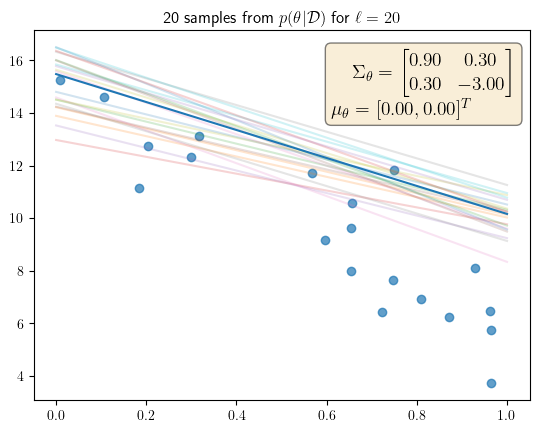
\includegraphics[width=0.8\textwidth]{assets/week1/fixed-prior-20-samples.png}
\end{subfigure}%
\begin{subfigure}{.5\textwidth}
  \centering
  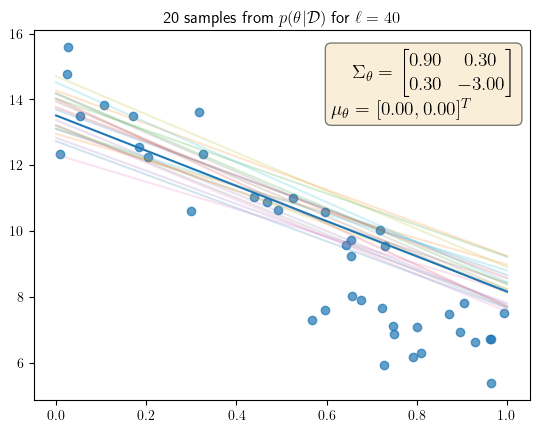
\includegraphics[width=0.8\textwidth]{assets/week1/fixed-prior-40-samples.png}
\end{subfigure}\\
\begin{subfigure}{1\textwidth}
  \centering
  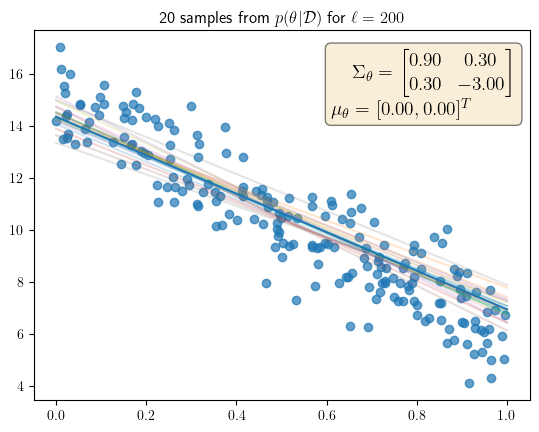
\includegraphics[width=0.4\textwidth]{assets/week1/fixed-prior-200-samples.png}
\end{subfigure}%
\caption{The model trained on data sets with 20, 40 and 200 data points respectively with a fixed prior. The blue line is $\mu_{\theta|\mathcal{D}}$.}
\label{fig:fixed-prior}
\end{figure}
\subsubsection{Variable prior}\todo{make explicit that it is $\Sigma_\theta$ that has been sampled}
\begin{figure}[H]
  \centering
  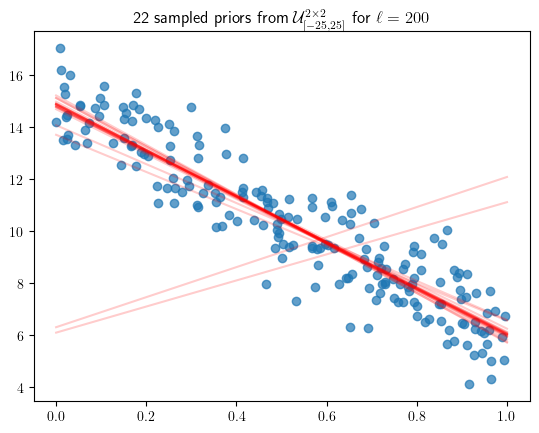
\includegraphics[width=0.6\textwidth]{assets/week1/variable-prior-fixed-samples.png}
  \caption{$\mu_{\theta | \mathcal{D}}$ for 22 sampled priors for $\ell=200$}
  \label{fig:variable-prior-fixed-samples}
\end{figure}

\subsubsection{Posterior predictive function}\todo{fix plot, maybe include $\Sigma_\theta$? include $\mu_{\theta|\mathcal{D}}$}
\begin{figure}[H]
  \centering
  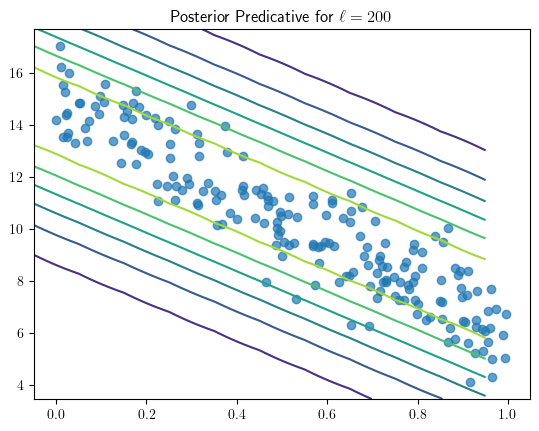
\includegraphics[width=0.6\textwidth]{assets/week1/posterior-predictive-1.png}
  \caption{Contour plot of the posterior predicative distribution for each value along the $x$ axis.}
  \label{fig:posterior-predictive-1}
\end{figure}
\subsection{Evaluation}
From figure \ref{fig:fixed-prior}, we see that the model is very sensitive to the amount of datapoints
in the dataset. The last plot with $\ell=200$ \todo{add sublabels}, we can see that larger amounts of 
data is not sufficient enough when the prior is bad - a good model should have both sufficient data and a good prior.\\
From figure \ref{fig:variable-prior-fixed-samples}, we can see that when data is sufficient, sampling random covariance matrices for the prior is likely to yield a good result.
From figure \ref{fig:posterior-predictive-1}, we can see that the posterior predictive distribution also looks to be quite representative of the data points, since the points become much more scarse as the become more distant from the yellow region.
